\documentclass[a4paper,10pt,twoside]{article}
%%%%%%%%%%% Packages %%%%%%%%%%
\usepackage[margin=1in]{geometry}
\usepackage{amsmath, amssymb,mathtools}
\usepackage{fancyhdr}
\usepackage{sectsty}
\usepackage{graphicx,wrapfig}
\usepackage{enumitem}
\usepackage{float}
\usepackage{braket}
\usepackage{bbm}
\usepackage{tikz,calc}

%%%%%%%%%%% Macros %%%%%%%%%%
\def \note#1 {\vspace{-1em}\paragraph{\bfseries #1}}
\def \dd {{\rm d}}
\def \id {{\mathbbm{1}}}
\def \order {\mathcal{O}}
\def\bquad{\mkern-18mu}
\DeclareMathOperator{\trace}{tr}
\DeclareMathOperator{\spanset}{span}

%%%%%%%%%%% Tikz Definitions %%%%%%%%%%
\usetikzlibrary{shapes, arrows,positioning,fit,automata}
\tikzstyle{plain} = [draw,thick,circle,inner sep=0,minimum size=0.5cm,font=\footnotesize]
\tikzstyle{mps} = [draw,thick,rectangle,rounded corners=.1cm,inner sep=0,minimum size=0.5cm]
\tikzstyle{mpo} = [draw,thick,circle,inner sep=0,minimum size=0.5cm]
\tikzstyle{index} = [-,thick,font=\footnotesize]
\tikzstyle{virtual} = [-,thick,dotted,font=\footnotesize]
\tikzstyle{site} = [draw,solid,circle,minimum size=2pt,inner sep=0pt,outer sep=0pt,fill=black]

\def \tu {0.25cm}

%%%%%%%%%%% Formatting %%%%%%%%%%
\pagestyle{fancy}
\renewcommand{\footrulewidth}{0.5pt}

\fancyhf{}
\lhead{22/07/2017}
\chead{Quantum Information Methods in Many-Body Physics}
\rhead{PH2269}
\lfoot{Giacomo Giudice~~~~giacomo.giudice@mpq.mpg.de}
\rfoot{Page \thepage}

\allsectionsfont{\normalfont\sffamily}

%%%%%%%%%%% Here Begins Document %%%%%%%%%%
\begin{document}
\title{\vspace{-1cm}\sffamily Solutions to Homework 7\vspace{-1cm}}
\author{}
\date{}
\maketitle
\thispagestyle{fancy}

\begin{section}{}
\paragraph{Introduction} 
Expanding the product 
\[
  \dots M^{[i]} M^{[i+1]} M^{[i+2]} M^{[i+3]} \dots  = 
  \dots
  \begin{pmatrix}
  \id & X_i + X_{i+1} + X_{i+2} + X_{i+3}  \\
  0 & \id
  \end{pmatrix} 
  \dots
\]
so, in order to close the product
\[
  M^{[1]}  = 
  \begin{pmatrix}
  \id & X_1 
  \end{pmatrix},
  \quad
  M^{[1]}  = 
  \begin{pmatrix}
   X_N \\
   \id
  \end{pmatrix}.
\]
Notice that in general, open boundary conditions imply that $M^{[1] i,j}_{a,b} = M^{i,j}_{1,b}$ and $M^{[N] i,j}_{a,b} = M^{i,j}_{a,\chi}$.
\paragraph{Nearest-Neighbor Interaction}  Compared to the previous example, we need to introduce an additional internal state
\begin{figure}[H]
  \centerline{
  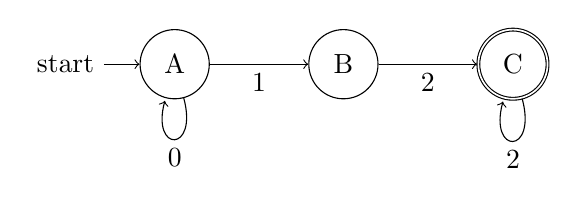
\begin{tikzpicture}[auto,node distance=5*\tu]
    \node[initial,state] (A) {A};
    \node[state,right=of A] (B) {B};
    \node[state,accepting,right=of B] (C) {C};
    \path[->] (A) edge[left] node[below]  {1} (B);
    \path[->] (B) edge[left] node[below]  {2} (C);
    \path[->] (A) edge[loop below] node[below]  {0} (A);
    \path[->] (C) edge[loop below] node[below]  {2} (C);
  \end{tikzpicture}
  }
\end{figure}
We need to add an additional rule to transition from an $\texttt{1}$ to the next $\texttt{1}$.
\[
  \left\{
  {
  \tikz[baseline=-0.5*\tu,node distance=\tu]{
      \node[mps]  (m) {};
      \draw[index] (m.north) -- +(0,\tu) node[above]{$\texttt{0}$};
      \draw[index] (m.west) -- +(-\tu,0) node[left]{0};
      \draw[index] (m.east) -- +(\tu,0) node[right]{0};
    }
  },
  {
  \tikz[baseline=-0.5*\tu,node distance=\tu]{
      \node[mps]  (m) {};
      \draw[index] (m.north) -- +(0,\tu) node[above]{$\texttt{1}$};
      \draw[index] (m.west) -- +(-\tu,0) node[left]{0};
      \draw[index] (m.east) -- +(\tu,0) node[right]{1};
    }
  },
  {
  \tikz[baseline=-0.5*\tu,node distance=\tu]{
      \node[mps]  (m) {};
      \draw[index] (m.north) -- +(0,\tu) node[above]{$\texttt{1}$};
      \draw[index] (m.west) -- +(-\tu,0) node[left]{1};
      \draw[index] (m.east) -- +(\tu,0) node[right]{2};
    }
  },
  {
  \tikz[baseline=-0.5*\tu,node distance=\tu]{
      \node[mps]  (m) {};
      \draw[index] (m.north) -- +(0,\tu) node[above]{$\texttt{0}$};
      \draw[index] (m.west) -- +(-\tu,0) node[left]{2};
      \draw[index] (m.east) -- +(\tu,0) node[right]{2};
    }
  }
  \right\}
\]
so we obtain the following MPO
\[
  M = 
  \begin{pmatrix}
  \id & X & 0 \\
  0 & 0 & X \\
  0 & 0 & \id
  \end{pmatrix} ,
\]

\paragraph{Heisenberg Model} Using the labels  $\id \sim \texttt{0}$, $\sigma^x \sim \texttt{1}$, $\sigma^x \sim \texttt{2}$, $\sigma^z \sim \texttt{3}$, we obtain the transitions map
\begin{figure}[H]
  \centerline{
  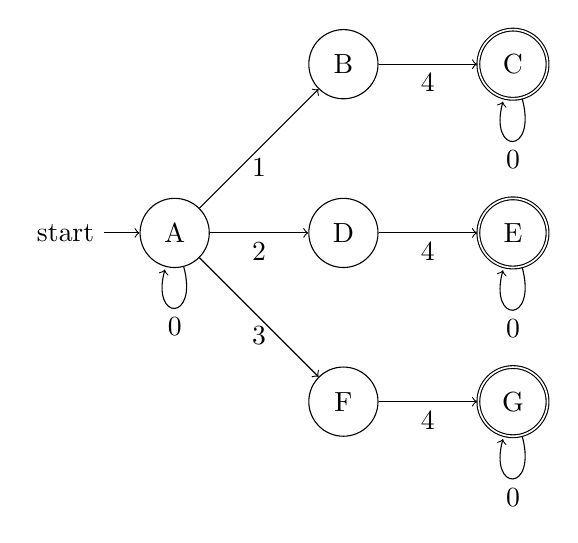
\begin{tikzpicture}[auto,node distance=5*\tu]
    \node[initial,state] (A) {A};
    \node[state,right=of A] (D) {D};
    \node[state,above=of D] (B) {B};
    \node[state,below=of D] (F) {F};
    \node[state,accepting,right=of B] (C) {C};
    \node[state,accepting,right=of D] (E) {E};
    \node[state,accepting,right=of F] (G) {G};
    \path[->] (A) edge[left] node[below]  {1} (B);
    \path[->] (B) edge[left] node[below]  {4} (C);
    \path[->] (A) edge[left] node[below]  {2} (D);
    \path[->] (D) edge[left] node[below]  {4} (E);
    \path[->] (A) edge[left] node[below]  {3} (F);
    \path[->] (F) edge[left] node[below]  {4} (G);
    \path[->] (A) edge[loop below] node[below]  {0} (A);
    \path[->] (C) edge[loop below] node[below]  {0} (C);
    \path[->] (E) edge[loop below] node[below]  {0} (E);
    \path[->] (G) edge[loop below] node[below]  {0} (G);
  \end{tikzpicture}
  }
\end{figure}
which corresponds to
\[
  M = 
  \begin{pmatrix}
  \id & \sigma^x & \sigma^y & \sigma^z & 0 \\
  0 & 0 & 0 & 0 & \sigma^z \\
  0 & 0 & 0 & 0 & \sigma^y \\
  0 & 0 & 0 & 0 & \sigma^x \\
   0 & 0 & 0 & 0 & \id
  \end{pmatrix}.
\]

\paragraph{Next Nearest-Neighbor Interaction}
In the following map we associate the weights $J_1$ with node C and $J_2$ with node E.
\begin{figure}[H]
  \centerline{
  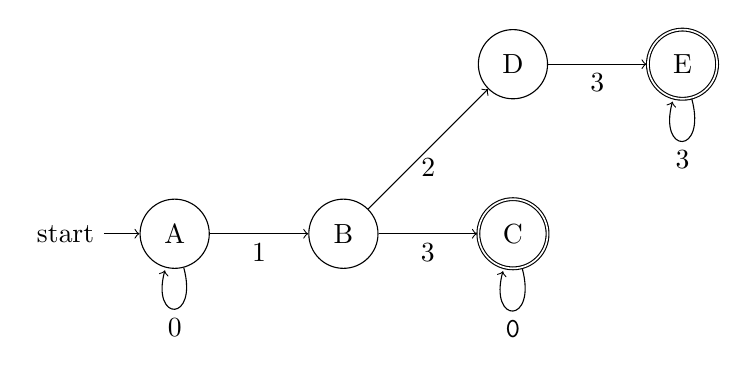
\begin{tikzpicture}[auto,node distance=5*\tu]
    \node[initial,state] (A) {A};
    \node[state,right=of A] (B) {B};
    \node[state,accepting,right=of B] (C) {C};
    \node[state,above=of C] (D) {D};
    \node[state,accepting,right=of D] (E) {E}; 
    \path[->] (A) edge[left] node[below]  {1} (B);
    \path[->] (B) edge[left] node[below]  {3} (C);
    \path[->] (B) edge[left] node[below]  {2} (D);
    \path[->] (D) edge[left] node[below]  {3} (E);
    \path[->] (A) edge[loop below] node[below]  {0} (A);
    \path[->] (C) edge[loop below] node[below]  {$\texttt{0}$} (C);
    \path[->] (E) edge[loop below] node[below]  {3} (E);
  \end{tikzpicture}
  }
\end{figure}
The MPO is then
\[
  M = 
  \begin{pmatrix}
  \id & Z & 0 & 0 \\
  0 & 0 & \id & J_1 Z \\
  0 & 0 & 0 & J_2 Z \\
  0 & 0 & 0 & \id
  \end{pmatrix} .
\]

\paragraph{Long-Range Interactions} By now you should be able to see that, in the finite state automaton picture, we obtain the picture below.
\begin{figure}[H]
  \centerline{
  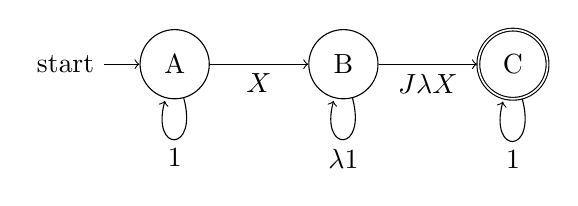
\begin{tikzpicture}[auto,node distance=5*\tu]
    \node[initial,state] (A) {A};
    \node[state,right=of A] (B) {B};
    \node[state,accepting,right=of B] (C) {C};
    \path[->] (A) edge[left] node[below]  {$X$} (B);
    \path[->] (B) edge[left] node[below]  {$J\lambda X$} (C);
    \path[->] (A) edge[loop below] node[below]  {$\id$} (A);
    \path[->] (B) edge[loop below] node[below]  {$\lambda\id$} (B);
    \path[->] (C) edge[loop below] node[below]  {$\id$} (C);
  \end{tikzpicture}
  }
\end{figure}
The interpretation is the following: once we hit a first $X$, we can propagate for any length $r$, each time hitting a $\lambda$ factor, until we end up in another $Z$. 
Once we end up in the second $X$, we do nothing.
The Hamiltonian is then the sum 
\[
  H = \sum_i \sum_{r>0} J \lambda^r X_i X_{i+r} .
\]
Defining $\lambda = e^{-1/\xi}$, we obtain the desired result.
\end{section}
\begin{section}{}
No solution is presented for this exercise.
\end{section}
\end{document}
%%%%%%%%%%% Here Ends Document %%%%%%%%%%
